\documentclass{beamer}
\usepackage{feynmp} % setup feynmp
\DeclareGraphicsRule{*}{mps}{*}{}
\usepackage{tikz}

% theme and general look
\usetheme{Rochester}
\usecolortheme{seahorse}

\setbeameroption{show notes}

% title information
\title[Muon Production and $A_{FB}$]{Muon Pair Production and Forward-Backward Asymmetry}
\author{L.~Siemens}


\begin{document}
\begin{fmffile}{presentation_mp} % begin feynmp environment

\begin{frame}
    \titlepage
    \note{\tableofcontents}
\end{frame}

\section{Setup}
\subsection{Montecarlo methods}
\begin{frame}{Mathematical Methods: Monte Carlo Integration}
    \begin{columns}
        \column{0.75\textwidth}
        average of a function $<f(x)> = \frac{1}{b-a}\int_a^b f(x)dx$

        \begin{block}{Estimate Integral}
            $\int_a^b f(x)dx = (b-a)<f(x)>$
        \end{block}
        \note[item]{Simples version of Monte Carlo integrationis derived directly from the difinition of the averag of thefuncktion on a domain}

        sampling uniformly at N random points

        \begin{block}{Estimated Error}
            $\sigma_{error} \propto 1/\sqrt{N}$
        \end{block}
        \note[item]{The error in the integral esimate is proportional to the standard error of the mean.}

        \note[item]{Notice that the error is indepedent of the dimension of the integral.}
        
        \column{0.25\textwidth}
    \end{columns}
\end{frame}

\begin{frame}{Mathematical Methods: Monte Carlo Sampling}{Rejection Sampling}
    \begin{columns}
        \column{0.75\textwidth}
        \begin{block}{Goal of Rejection Sampling}
            Sample the distribution $f(x)$ on the domain $[a, b]$
        \end{block}

        \begin{enumerate}
            \item Uniformly sample $[a, b] \times [0, 1]$ labeling points $(x_i, v_i)$
            \item Reject any sample with $v_i > f(x_i)/f_{max}$
            \item The remaining $x_i$ values follow the distribution $f(x)$
        \end{enumerate}
        \note[item]{Note that the maximum of the function n the domain must be known beforehand.}
        \column{0.25\textwidth}
    \end{columns}
\end{frame}

\subsection{Equations and differential cross section}
\begin{frame}{Muon Pair Production: $e^+ + e^- \rightarrow \mu^+ + \mu^-$}
    \begin{columns}
        \column{0.60\textwidth}
        \begin{block}{Expected number of events}
            $N_{exp} = L_{int} \cdot \sigma_{tot}$
        \end{block}
        \note[item]{Expected number of events from time integrated luminosity and the total cross section}

        In center of momentum frame and using the relitivistic limit

        \begin{itemize}
            \item $p_1^{\mu} = (E, 0, 0, E)^{\mu}$
            \item $p_3^{\mu} = (E, E\sin(\theta), 0, E\cos(\theta))^{\mu}$
        \end{itemize}
        \note[item]{Note that the angle $\theta$ is the angle of the out going muon relative to the incoming electron.}

        \column{0.40\textwidth}
        \begin{fmfgraph*}(100, 80)
            \fmfleft{i2,i1}
            \fmfright{o4,o3}
            \fmf{fermion}{i1,v1,i2}
            \fmf{fermion}{o4,v2,o3}
            \fmf{photon, label=$\gamma,,Z^0$}{v1,v2}
            \fmflabel{$e$}{i2}
            \fmflabel{$\mu$}{o4}
            % Momentum arrows
            \fmfcmd{%
                vardef normal (expr p, mag) = 
                    (1, 0)
                    rotated (90 + angle direction 0.5*length(p) of p)
                    scaled mag
                enddef;
                % draw momentum arrow on left side of ray
                style_def marrowl expr p =
                    drawarrow subpath (1/4, 3/4) of p
                    shifted normal (p, 6)
                    withpen pencircle scaled 0.4;
                enddef;
                % draw momentum arrow on right side of ray
                style_def marrowr expr p =
                    drawarrow subpath (1/4, 3/4) of p
                    shifted normal (p, -6)
                    withpen pencircle scaled 0.4;
                enddef;}
            \fmf{marrowr, label=$p_1$, tension=0}{i1,v1}
            \fmf{marrowr, label=$p_3$, tension=0}{v2,o3}
        \end{fmfgraph*}

        \begin{figure}
            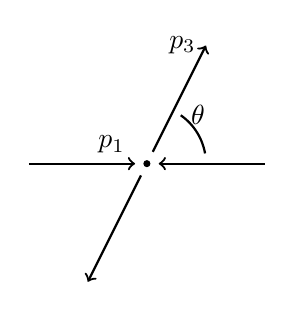
\begin{tikzpicture}[scale=1.5]
                \draw [thick,->] (-1,0) -- (-0.1,0) node[above left] {$p_1$};
                \draw [thick,<-] (0.1,0) -- (1,0);
                \draw [thick,->] (0.05,0.1) -- (0.5,1) node[left] {$p_3$};
                \draw [thick,domain=10:55] plot ({0.5*cos(\x)}, {0.5*sin(\x)}) node[right] {$\theta$};
                \draw [thick,<-] (-0.5,-1) -- (-0.05,-0.1);
                \draw [fill] (0,0) circle [radius=0.025];
            \end{tikzpicture}
        \end{figure}
    \end{columns}
\end{frame}

\begin{frame}{Differential Cross Section}
    Diagram amplitudes $A_{\gamma}$, $A_{Z}$

    \begin{block}{$Z^0$ Feynman rules}
        \begin{columns}
            \column{0.4\textwidth}
            \centering
            \begin{block}{Propagator}
                \centering
                $\frac{-i(g_{\mu \nu} - q_{\mu}q_{\nu}/M_Z^2)}{q^2 - M_z^2 + iM_Z \Gamma_Z}$
                \note[item]{The $Z^0$ boson propegator is that of a massive spin 1 particle}
                \note[item]{The term $iM_Z\Gamma_Z$ is due to decay of the $Z^0$ boson}
            \end{block}

            \column{0.4\textwidth}
            \centering
            \begin{block}{Vertex factor}
                \centering
                $\frac{-ig_Z}{2}\gamma^{\mu}(c_v^f - c_A^f\gamma^5)$
                \note[item]{The term $\gamma^5$ in the vertex factor lads to the antisymmetric factors of $\cos(\theta)$ in the spin averaged amplitude squared.}
            \end{block}
        \end{columns}
    \end{block}

    Spin averaged amplitude squared $<|A_{\gamma}|^2>$, $<|A_Z|^2>$ $<A_{cross}^2>$
    \note[item]{All three terms have different dependence on the energy.}

    \begin{alertblock}{Angular dependence of terms}
        \begin{itemize}
            \item $<|A_{\gamma}|^2> \propto 1 + \cos^2(\theta)$
            \item $<|A_Z|^2> \propto 1 + \cos^2(\theta) + a\cos(\theta)$
            \item $<A_{cross}^2> \propto 1 + \cos^2(\theta) + b\cos(\theta)$
        \end{itemize}
        \note[item]{The factors $a$ and $b$ have different dependence on the vector-axial coupings}
    \end{alertblock}
\end{frame}

\subsection{Simulation Procedure}
\begin{frame}{Simulation Outline}
    \begin{enumerate}
        \item Estimate $\sigma_{tot}$ and the maximum of $\frac{d\sigma}{d\Omega}\sin(\theta)$ using montecarlo integration
        \note[item]{Calculate the maximum of $\frac{d\sigma}{d\Omega}\sin(\theta)$ using the samples of the function takin in the Monte Carlo integration}

        \item Calculate expected number of events $N_{avg} = L_{int} \cdot \sigma_{tot}$
        \item Sample one value, $N$, from the Poisson distribution with mean $N_{avg}$
        \note[item]{Note, using the Poisson distribution is only nessisary if the number of expected events $N_{avg}$ is small. TODO rephrase}

        \item Use Monte Carlo sampling to get $N$ random samples with distribution determined by $\frac{d\sigma}{d\Omega}$
        \note[item]{This simulatates muon pair production events at a fixed eerngy with out accounting for effects in the detector . . .}
        \item Calculate $p_3^{\mu}$ from $E$ and $\theta$ for each sample and save to disk
    \end{enumerate}
    \note[item]{With multiple runs at fixed integrated luminosity at a veriety of energies. TODO finish}
\end{frame}

\section{The Data}
\subsection{Angular Distribution}
\subsection{Cross Section vs Energy}
\subsection{Forward Backward Asymmetry Equations (Optional?)}
\subsection{Forward Backward Asymmetry}
\begin{frame}
    TODO fill in frames for data and results
    \note[item]{Talk about the $A_{FB}$ asymmetry}
\end{frame}

\end{fmffile}
\end{document}
